\documentclass{hertieteaching}
\usepackage{cancel}
\usepackage{hyperref}

\title{Sentiment}

\begin{document}

\maketitle

\begin{frame}{Sentiment analysis}

\begin{itemize}
  \item Are these documents getting more positive (negative) over time?
  \item Do people like this product (party, person)?
\end{itemize}

My unpopular opinion (which you need not share): Not very interesting, and really a field of its own\ldots
\begin{itemize}
  \item An active applied subfield of computer science
  \item Some applications in social science
  \item Huuuuuge applications in marketing
\end{itemize}

\pause

Theoretically ambiguous: mostly mixes positive affect, optimism, happiness, etc. and their opposites together into
\begin{itemize}
  \item a continuous measure: negative $\longleftrightarrow$ positive
  \item an ordinal scale, e.g. 0-5 stars
  \item a classification, e.g 0 (`negative') or 1 (`positive')
\end{itemize}
\end{frame}

\begin{frame}{Measuring sentiment}

Consequently we can get sentiment measures in a lot of ways
\begin{itemize}
  \item Dictionary models
  \item Scaling models
  \item Classification models
\end{itemize}
We'll consider a mix of the first two and the third

Why a mix?
\begin{itemize}
  \item In dictionary applications sentiment is operationalised as the \textit{relative prevalence of positive over negative} terms or mentions
  \item First run dictionary to get `pos' and `neg' counts, then transform, e.g. as a smoothed logit 
$$
\log\left(\frac{\text{pos} + \alpha}{\text{neg} + \alpha}\right)
$$
which \textsf{quanteda} calls \textit{polarity}
\end{itemize}

\end{frame}

\begin{frame}{Dictionaries vs handcoding}

\centerline{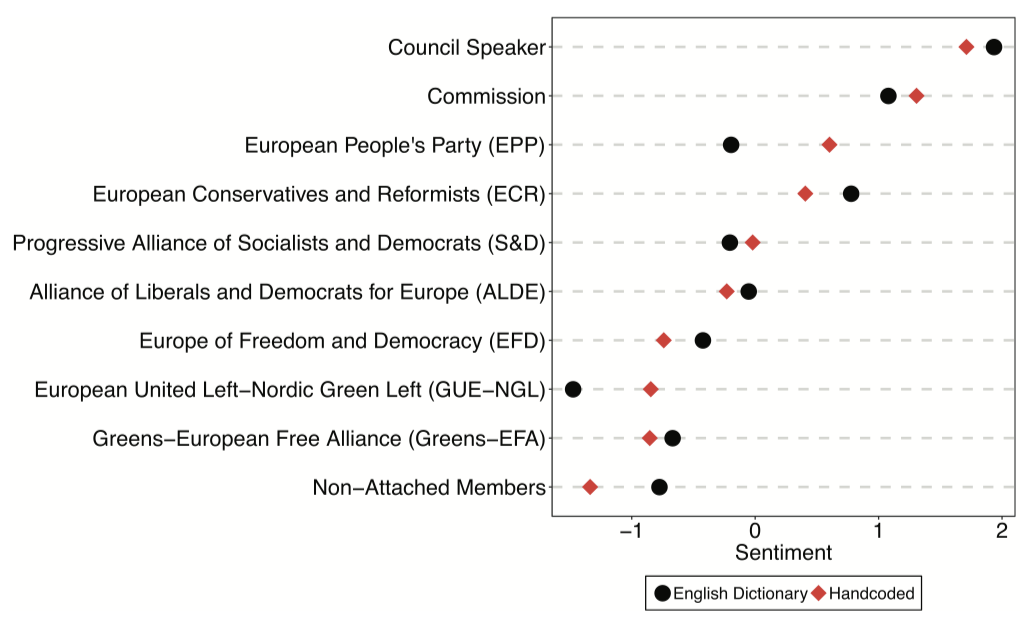
\includegraphics[scale=0.5]{pictures/multilingual-sent-ep}}

EP State of the Union debate 2010 using (english) Lexicoder dictionaries and polarity measure \parencite{Proksch.etal2019}
\end{frame}

\begin{frame}{Sentiment and government vs opposition}

\centerline{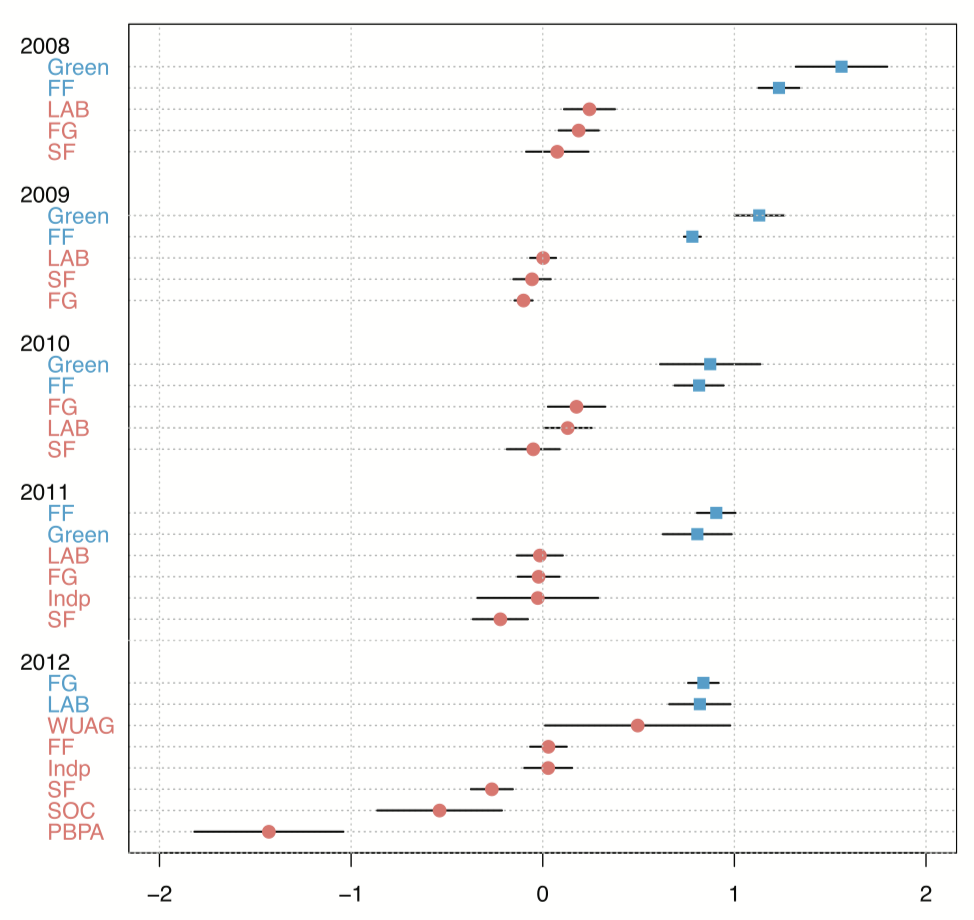
\includegraphics[scale=0.4]{pictures/multilingual-sent-ie}}

Budget debates in Ireland \parencite{Proksch.etal2019}

\end{frame}

\begin{frame}{Sentiment over time}

\centerline{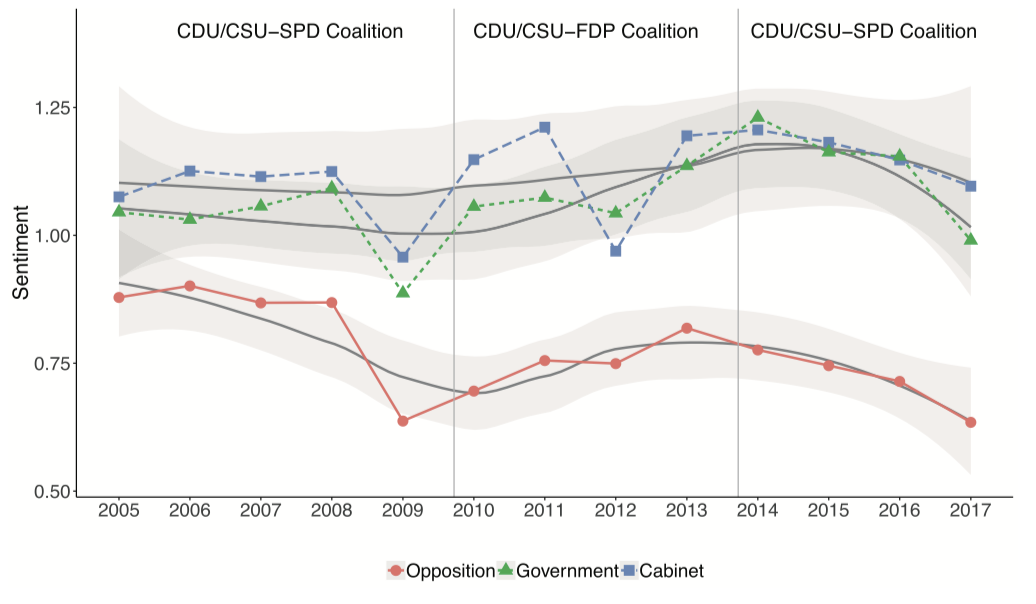
\includegraphics[scale=0.5]{pictures/multilingual-sent-de}}

Sentiment on government bills in the German legislature, 2015-2017 \parencite{Proksch.etal2019}

\end{frame}
\begin{frame}{Sentiment as cross-linguistic anchoring}

\begin{itemize}
  \item Text comparisons across languages is just hard
  \item Hand translation is often not available, expensive, and difficult to evaluate
  \item Maybe tracking some basic human interaction features is easier to compare?
\end{itemize}
\textcite{Proksch.etal2019} hoped so. I'm not sure if we were right.

\bigskip
\centerline{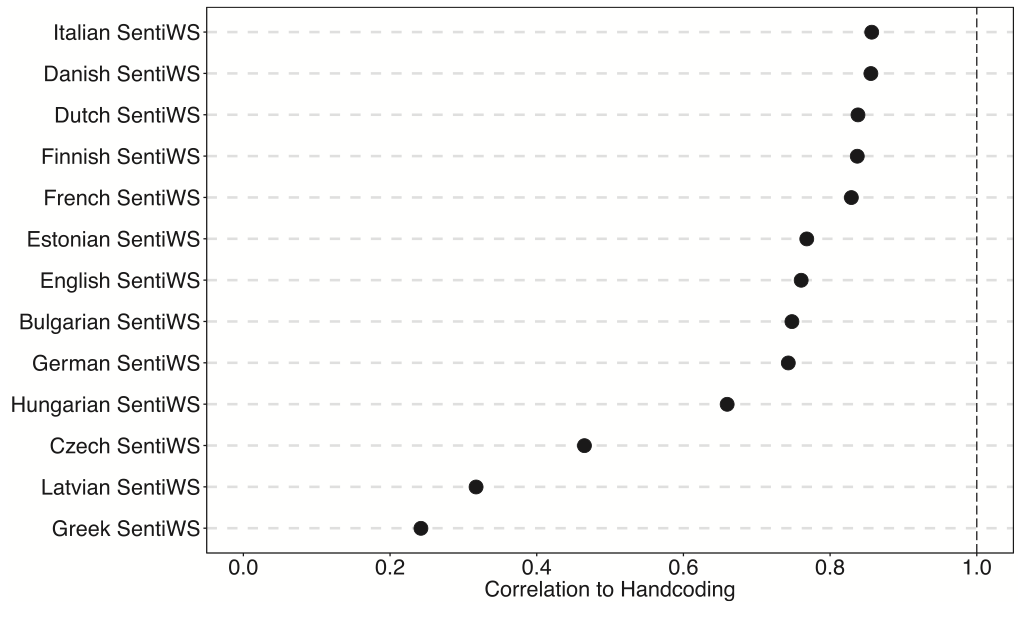
\includegraphics[scale=0.3]{pictures/multilingual-sent-comp}}

Note: there's still translation happening, but of fewer `easier' terms from a dictionary
\end{frame}

\begin{frame}{Dictionaries}

Lots of dictionaries out there. \textsf{quanteda.sentiment} (from github) contains several
\begin{itemize}
  \item \textcite{Nielsen2011} new Affective Norms for English Words (ANEW)
  \item \textcite{Stone.etal1966} Augmented General Inquirer
  \item \textcite{Hu.Liu2004} Positive and negative terms
  \item \textcite{Loughran.Mcdonald2011} Sentiment Word Lists
  \item \textcite{Albugh.etal2013} Lexicoder Sentiment Dictionary (2015)
  \item \textcite{Mohammad.Turney2013} NRC Word-Emotion Association Lexicon
  \item \textcite{Rauh2018} German Political Sentiment Dictionary
  \item \textcite{Remus.etal2010} `Senti Wortschatz' (SentiWS) 
\end{itemize}

  
\end{frame}
\begin{frame}{Classification}

Word lists are necessarily domain \textit{un}specific

If we need a sense of sentiment specific to a particular discourse or institution, then 
\begin{itemize}
  \item Hand construct a dictionary
  \item Categorize a set of examples and try to train a classifier
\end{itemize}

Rather generally

\bigskip
\centerline{expert constructed dictionary ~~\textit{beats}~~ classifier ~~\textit{beats}~~ general purpose dictionary}

but your mileage may vary\ldots 

\end{frame}

\begin{frame}{Classification}

The easiest way to get a practical feel for how a classifier would work is to make one work

Let's do that next\ldots   
\end{frame}




\begin{frame}[allowframebreaks]
\frametitle{References}
\printbibliography	
\end{frame}

\end{document}
